% Created 2018-04-29 Sun 20:33
\documentclass[11pt]{article}
\usepackage[utf8]{inputenc}
\usepackage[T1]{fontenc}
\usepackage{fixltx2e}
\usepackage{graphicx}
\usepackage{longtable}
\usepackage{float}
\usepackage{wrapfig}
\usepackage{rotating}
\usepackage[normalem]{ulem}
\usepackage{amsmath}
\usepackage{textcomp}
\usepackage{marvosym}
\usepackage{wasysym}
\usepackage{amssymb}
\usepackage{hyperref}
\tolerance=1000
\usepackage{hyperref}
\usepackage{cleveref}
\usepackage{xcolor}
\hypersetup{colorlinks, linkcolor={red!50!black},citecolor={blue!50!black}, urlcolor={blue!80!black}}
\usepackage{amsmath}
\author{Zhao Wei}
\date{\today}
\title{COSC420 Neural Network Assignment Report}
\hypersetup{
  pdfkeywords={},
  pdfsubject={},
  pdfcreator={Emacs 25.3.1 (Org mode 8.2.10)}}
\begin{document}

\maketitle
\tableofcontents


\section{Introduction}
\label{sec-1}
My neural network is a simple fully connected feedforward network with just one hidden layer. The number of input, hidden and output units can be specified through a \texttt{param.txt} file. The program reads input pattern and teaching input pattern from \texttt{input.txt} and \texttt{teaching\_input.txt} respectively. 

This report describes the implementation of my neural network and some tests which use the dataset from cosc420 web page. 
\section{Background}
\label{sec-2}
My neural network is a fully connected. It implements the general delta rule for backpropagation and uses sigmoid function as activation function. During initialization, if the number of patterns in data is 150(which is iris flow dataset), then it randomly select 100 patterns as the training dataset, the rest 50 patterns will be used as testing dataset. If the dataset is very simple one, it will not divide the dataset into training and testing, since the dataset is so small, and we need every pattern in it to train. My training uses the online approach. It means the backpropagation will be done for every input pattern. Also, I shuffle the dataset before every epoch.

My experiments focus on the changes of learning rate, number of hidden units and using testing accuracy as learning criteria.

\section{Experiment}
\label{sec-3}
\subsection{Change the learning rate}
\label{sec-3-1}
Learning rate plays an important role since it appears in almost every machine learning algorithm. How to set it is based on some heuristic, so I want to see the effect of it on my neural network. I use the iris dataset and collect training epochs while changing the learning rate with a different value.

Table \ref{table-epochs-needed} shows the epochs needed to train my neural network to \texttt{learning\_criteria (popErr) = 0.05} with different learning rate on iris dataset. Other parameters are the same including learning momentum is 0.9.

\begin{table}[htb]
\caption{table shows the epochs needed to reach a popErr criteria, with different learning rate.  \label{table-epochs-needed}}
\centering
\begin{tabular}{rrrrrrr}
id & r=0.2 & r=0.15 & r=0.13 & r=0.11 & r=0.08 & r=0.05\\
\hline
1 & 66 & 55 & 117 & 5705 & 229 & 4441\\
2 & 183 & 301 & N/A & 1571 & 864 & 2375\\
3 & 179 & 216 & 178 & 228 & 310 & 1463\\
4 & 217 & 105 & 205 & N/A & 259 & 7884\\
5 & 513 & 135 & 1922 & 237 & 898 & 379\\
6 & 92 & N/A & 169 & 1791 & 3015 & 1124\\
7 & N/A & 172 & 755 & 2318 & N/A & 1111\\
8 & 6748 & 170 & 124 & 226 & 1851 & 269\\
9 & 842 & 338 & 313 & N/A & 2429 & N/A\\
10 & 75 & 155 & 7656 & 566 & 463 & 309\\
11 & 49 & 466 & N/A & 193 & 258 & 383\\
12 & 68 & 2233 & 123 & N/A & 121 & 719\\
13 & 344 & 1872 & 176 & 608 & 167 & 621\\
14 & 43 & 80 & 289 & 98 & 388 & 250\\
15 & 81 & 6862 & 5623 & 128 & 255 & 325\\
16 & 128 & 69 & 179 & 234 & 214 & N/A\\
17 & N/A & 80 & 1077 & 8795 & 831 & 298\\
18 & 3805 & 211 & 262 & 241 & 1386 & 273\\
19 & 3100 & 186 & 110 & 192 & 949 & 617\\
20 & 52 & N/A & 119 & 2885 & 365 & 341\\
21 & 151 & 87 & 483 & 152 & 596 & 1590\\
22 & 3956 & 37137 & 308 & 197 & 223 & 387\\
23 & 48 & 104 & 18465 & 232 & N/A & 1314\\
24 & 83 & 123 & N/A & 122 & 12753 & 279\\
25 & 3100 & 587 & 38938 & N/A & 489 & 171\\
26 & 310 & 130 & 181 & 697 & 479 & 676\\
27 & 151 & 201 & 241 & 150 & 14169 & 6996\\
28 & 204 & 212 & 543 & 243 & 1258 & 19315\\
29 & 703 & 128 & 726 & 148 & 847 & 731\\
30 & 16186 & 3912 & 321 & 241 & 565 & 2763\\
31 & 185 & 182 & 430 & 199 & 2098 & 2420\\
32 & 125 & 312 & 262 & 346 & N/A & 3022\\
33 & 304 & 403 & 647 & 515 & 580 & N/A\\
34 & 61 & 539 & 102 & 798 & N/A & N/A\\
35 & 104 & N/A & 172 & 183 & 236 & 1562\\
\hline
Times of N/A & 2 & 3 & 3 & 4 & 4 & 4\\
Mean & 663.138 & 371.077 & 608.769 & 436.522 & 715.391 & 1078.652\\
\end{tabular}
\end{table}

\begin{itemize}
\item Because sometimes it shows no signs to reach the learning criteria, I have to cancel the training. And the corresponding cell in the table has recorded as N/A.
\item To collect the statistics, I get rid of the corresponding number of N/A for minimum and maximum epochs in each column. For example, there are 2 N/A for r=0.2, so when I compute the average epochs, I will not consider the two smallest and two maximum epochs in the r=0.2 column.
\item The final average value is filled in the final row. After plotting it out, it is shown in figure \ref{fig-average-epochs}. It shows that the general average epochs needed are increasing  while the learning rate is decreasing.
\begin{figure}[htb]
\centering
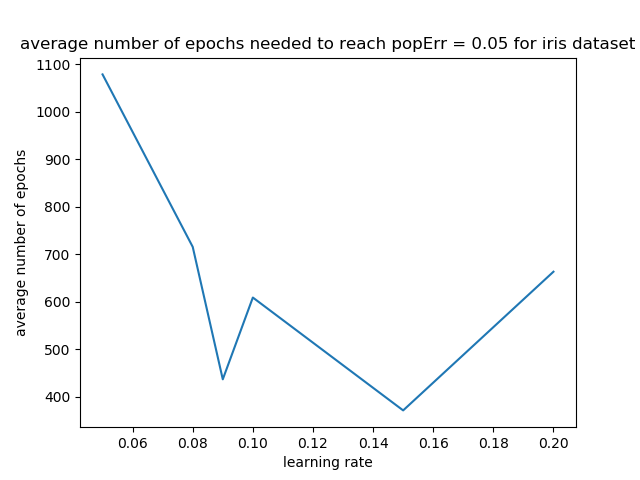
\includegraphics[width=.9\linewidth]{./average_epochs.png}
\caption{shows average epochs needed to reach popErr = 0.05 for training on iris dataset with 6 hidden units \label{fig-average-epochs}}
\end{figure}
\end{itemize}


\subsubsection{Using testing accuracy as criteria}
\label{sec-3-1-1}
Though dozens of experiments, I found out the popErr sometimes could not represent the real effect of learning. After all, we need to generalize well on the testing dataset to confirm the neural network is working which is evaluated by the testing accuracy.  

So, using popErr as learning criteria is not sufficient. Furthermore, accuracy could fluctuate a lot with small changes on popErr, see figure \ref{fig-iris-fluctuate}.
\begin{figure}[htb]
\centering
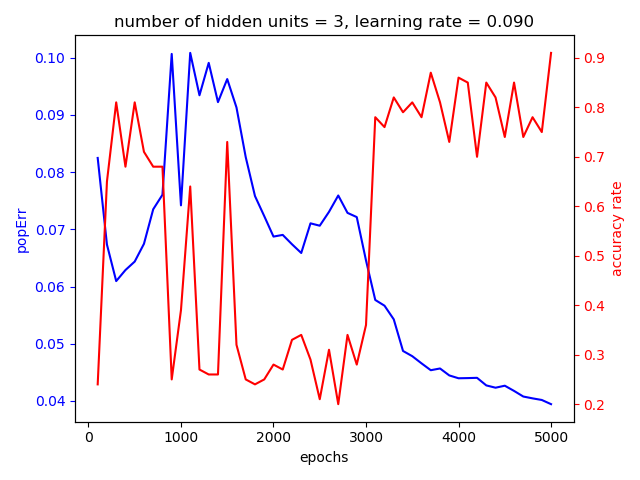
\includegraphics[width=.9\linewidth]{./popErr_vs_accuracy_on_iris_accuracy_fluctuate_with_popErr.png}
\caption{training on iris dataset, shows accuracy fluctuate a lot with small changes on the popErr  \label{fig-iris-fluctuate}}
\end{figure}

Before collecting the testing accuracy, I need to define what is True or False for my learning output. Because the teaching input is integer vector which is used to define classes, there will always some differences between my NN's output and the ground truth. So I define the fit criteria = 0.4, it means if the corresponding attribute between teaching input and NN's out is greater than 0.4, I consider the output is False. For example, during testing I randomly pick a pattern and compare the corresponding attribute difference:
\begin{verbatim}
the input is: [0.137 0.584 0.102 0.043]
the teaching input is: [1. 0. 0.]
the output is: [0.84735159 0.45242708 0.00200901]
the differences between corresponding attribute is > 0.45, so decide it is False.
\end{verbatim}

This simple scheme will help me to compare the proportion of each attribute to decide if it is a correct classification. The reason this works because in the teaching input, there is only 1 attribute will be marked as 1 and the rest is 0.

The accuracy is computed by (the number of True) / (the number of total tested patters). In my program, I will randomly select 100 patterns from testing set. By using testing accuracy as the learning criteria, it alleviates the problem of adjusting the small popErr.

\subsection{Change the number of hidden units}
\label{sec-3-2}
Though experiment, I can feel that the number of hidden units indeed plays the key role. Since the hidden units control the ability to abstract the patterns from the environment.
\subsubsection{Change the number of hidden units for encoder dataset}
\label{sec-3-2-1}
Currently, I couldn't get a good result on encoder dataset. I have tried increasing the number of hidden units, but it does not improve the accuracy significantly. Its accuracy is always around 0.125 which indicates the network is doing arbitrary classification.


\subsubsection{Change the number of hidden units for iris dataset}
\label{sec-3-2-2}
For using the same setting except for the number of hidden units, I train the neural network on iris dataset with multiple time to collect the epochs needed to reach accuracy = 0.9. I record down the result in the table \ref{table-epochs-needed-for-accuracy}. It is clear to see that more hidden units could improve the performance of a neural network. The fluctuation of training epochs is much smaller on the network with 6 hidden units and overall the training time is smaller than using 3 hidden units. Figure \ref{fig-iris-hidden-3-long-process}  shows a hard training process with 3 hidden units.

\begin{table}[htb]
\caption{epochs needed for training on iris dataset to reach accuracy = 0.9 with different hidden units.  \label{table-epochs-needed-for-accuracy}}
\centering
\begin{tabular}{rrr}
id & 3 hidden units & 6 hidden units\\
\hline
1 & 1000 & 200\\
2 & 13700 & 900\\
3 & 1900 & 300\\
4 & 200 & 400\\
5 & 5700 & 800\\
6 & 400 & 300\\
7 & 1800 & 700\\
8 & 500 & 200\\
9 & 1700 & 1200\\
10 & 5000 & 1400\\
11 & 200 & 1400\\
12 & 3400 & 3600\\
13 & 3100 & 300\\
14 & 700 & 200\\
15 & N/A & 300\\
16 & 700 & 900\\
17 & N/A & 200\\
18 & 12000 & 200\\
19 & 4700 & 300\\
20 & 300 & 600\\
\hline
time of N/A & 2 & 0\\
mean & 2207.142 & 720\\
\end{tabular}
\end{table}

\begin{figure}[htb]
\centering
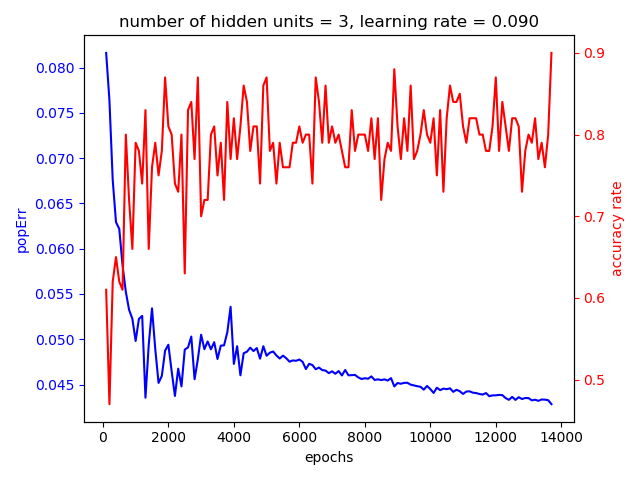
\includegraphics[width=.9\linewidth]{./popErr_vs_accuracy_on_iris_3hidden_hard.png}
\caption{Training on iris dataset with 3 hidden to reach accuracy = 0.9 could be a long process. \label{fig-iris-hidden-3-long-process}}
\end{figure}

\section{Discussion}
\label{sec-4}
Though the experiments on training my neural network, I notice several points:
\begin{enumerate}
\item Larger learning rate can reduce popErr faster than smaller learning rate. However, popErr is hard to use as a learning criterion, so I defined the testing accuracy criteria. And find out smaller learning rate can usually reach high accuracy. The reason is to get a high accuracy, the popErr need to be reduced to a smaller value, but big learning rate makes the neural network oscillate on the error surface and could not settle down to the minimum. I personally found 0.09 is a good choice, it just works well during the training.
\item Increase the number of hidden units could boost the learning capacity of a neural network. Such as training on iris dataset, when I increase the number of hidden units from 3 to 6, the learning becomes more steady and the average epochs needed to reach that accuracy is also decreased.
\item I have train the neural network on multiple datasets. The general result is summarised as follow:
\begin{itemize}
\item 5:3:5: accuracy fluctuated between 0.5 and 0 since it only has two patterns. It is very hard to reach high accuracy. After increasing hidden units to 5, accuracy fluctuated less and reached 1.0, see figure \ref{fig-535}.
\begin{figure}[htb]
\centering
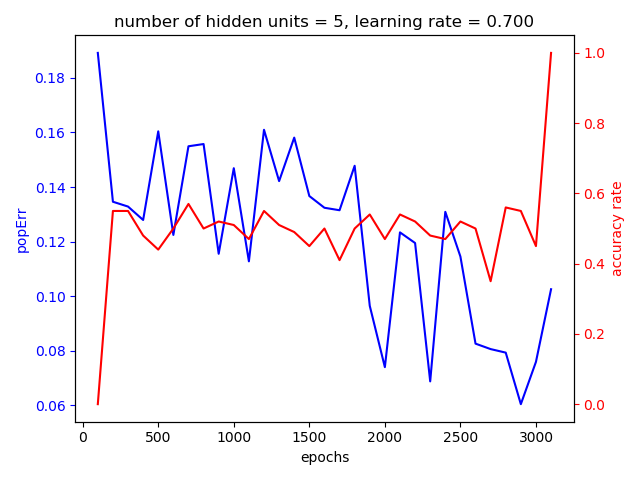
\includegraphics[width=.9\linewidth]{./popErr_vs_accuracy_on_535.png}
\caption{training on dataset 5:3:5, with extra hidden units, reach accuracy = 1.0 \label{fig-535}}
\end{figure}
\item 2:2:1, xor: My neural network could achieve accuracy = 1.0 using the default setting relative easily.
\item 3:3:1: accuracy fluctuated a lot, makes it hard to get a high accuracy. After increasing hidden units to 6, accuracy fluctuate less and reached to high accuracy, see figure \ref{fig-331}.
\begin{figure}[htb]
\centering
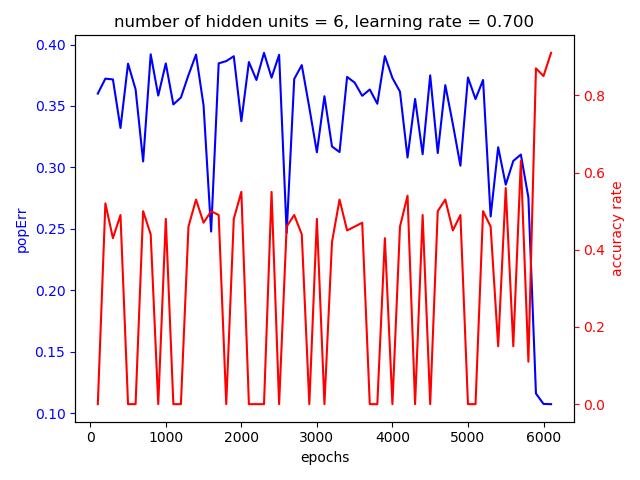
\includegraphics[width=.9\linewidth]{./popErr_vs_accuracy_on_331_dataset.png}
\caption{training on dataset 3:3:1, with extra hidden units, reach accuracy above 0.9 \label{fig-331}}
\end{figure}
\item 4:4:1: Using default setting and after a long time training, its accuracy fluctuated to reach 0.95, see figure \ref{fig-441}.
\begin{figure}[htb]
\centering
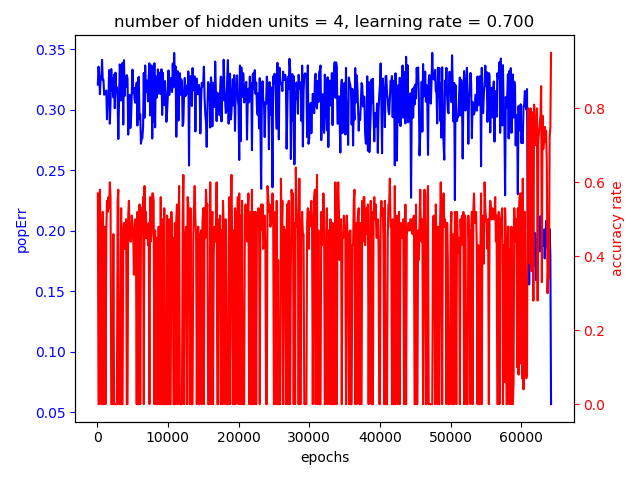
\includegraphics[width=.9\linewidth]{./popErr_vs_accuracy_on_441.png}
\caption{It is lucky that after a long time training, the neural network achieved a high accuracy on 4:4:1 dataset  \label{fig-441}}
\end{figure}
\item 8:3:8: The popErr could be reduced to 0.09, the accuracy is around 0.11 \textasciitilde{} 0.14.
\item iris: After increasing hidden units to 6, the training to high accuracy becomes faster and more steady.
\end{itemize}

\item The initial state of a neural network is very important. Sometimes, same settings with different initial weights will behave very differently. For example, figure \ref{fig-iris-hard-training} shows a hard training process on iris dataset for accuracy = 0.9 with 3 hidden units. 
\begin{figure}[htb]
\centering
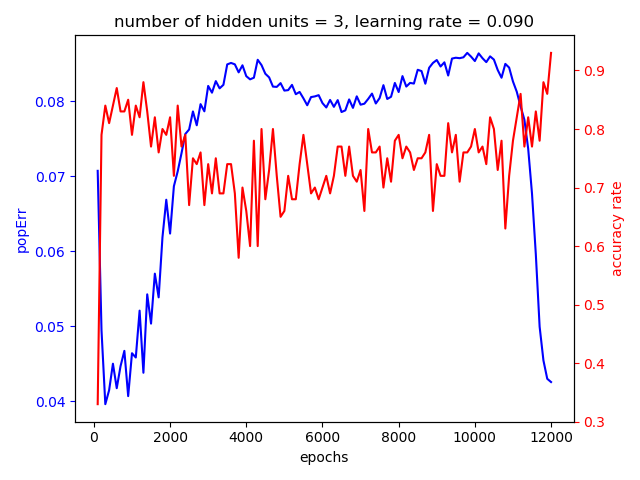
\includegraphics[width=.9\linewidth]{./popErr_vs_accuracy_on_iris_hard_training.png}
\caption{a very hard training on iris dataset with 3 hidden units \label{fig-iris-hard-training}}
\end{figure}
\end{enumerate}


In general, it is useful to define different kinds of method to guide the network training to reach a result you expected. But it is hard to specify a uniform rule so that as long as you follow that you could reach the goal. Furthermore, if the training of neural network is like walking on the error surface to reach the global lowest place, then whether you could reach there not only depend on the method you used but also depends on the initial place you start. That is very hard to control. That's why there is big variance on my training epochs with same settings. At last, after you designing everything, you just need to wait and have faith in your neural network, such as the case shown in figure \ref{fig-441}.

\section{Appendix}
\label{sec-5}
The whole program is implemented with Python 2.7.14. It relies on Numpy for dataset manipulation and Pyplot for plotting the graph.
\subsection{The component of the program}
\label{sec-5-1}
\begin{itemize}
\item NeuralNetwork.py, is the model which contains the class NN for abstract a fully connected neural network.
\item main.py, is the controller. It contains the main entry point to call NN's different method based on user's input.
\item It also contains three .txt file for storing the information about parameters, input, and teaching input respectively.
\end{itemize}
\subsection{Usage}
\label{sec-5-2}
\subsubsection{How to run the program}
\label{sec-5-2-1}
Run \texttt{python ./main} on commmand-line.
The program will try to load 3 files in the same directory: \texttt{param.txt}, \texttt{input.txt} and \texttt{teaching\_input.txt}. You could also changes the corresponding code within \texttt{main.py}:
\begin{verbatim}
def initialize(self):
    params = np.loadtxt('param.txt')
    inputs = np.loadtxt('input.txt')
    teachingInput = np.loadtxt('teaching_input.txt')
\end{verbatim}
\subsubsection{How to use the program}
\label{sec-5-2-2}
After starting the program, it will keep running in a loop to wait for the user's input:
\begin{verbatim}
Please input 0 - 9 to select:
1 : initialize
2 : teach 100 epochs
3 : teach until accuracy >= 0.90 during testing
4 : teach to criteria
5 : randomly select one patter to test
6 : show weights
7 : run 100 test and collect training result
8 : check hidden units
9 : check settings without re-initialize the net
0 : quit
your choice =>
\end{verbatim}

\begin{itemize}
\item You need to \textbf{first} initialize the neural network, choose 1.
\item Then, you could choose other options. Notice, the option 3 and 4 will keep training the neural network until it reaches the pre-specific settings. It could not be stopped during the process.
\item If you want to start another training, you could restart the program or choose option 1 to reset the whole program to initial state.
\end{itemize}
% Emacs 25.3.1 (Org mode 8.2.10)
\end{document}